\chapter{Framework}

% **************************** Define Graphics Path **************************
\ifpdf
\graphicspath{{Chapter3/Figs/Raster/}{Chapter3/Figs/PDF/}{Chapter3/Figs/}}
\else
\graphicspath{{Chapter3/Figs/Vector/}{Chapter3/Figs/}}
\fi
In this chapter we present the basic framework of our vessel segmentation method. We start by setting up the various notations used throughout the chapter and give an overview about how the framework is applied. Next we discuss the two different models applied in the framework. This forms the core of this thesis and represents the major work done. At last we mention the various datasets utilized to test our models. In the next chapter we experimentally evaluate the models.\\
\section{Vessel segmentation Framework}
We start by defining the basic notations and methods. The input to our vessel segmentation framework is a training set composed of fundus images and their corresponding segmentation or label maps. The collection of fundus images is represented by $\bar{I} = (I^{(1)},I^{(2)}...., I^{(n)} )$  and their corresponding ground truth segmentation maps as $\bar{S} = (S^{(1)},S^{(2)}...., S^{(n)} )$. Each given image is of size M x N.
For simplicity, in the rest of the section a we would refer an image as I and its segmentation map as S. We also assume that the image I is a single channel image.\\

We can represent an image as a collection of overlapping patches computed around every pixel take at center. A patch is of size $\sqrt{n}$ x $\sqrt{n}$ unless otherwise noted. We represent a patch centered at location (x ,y) as $p_{x,y}$, and patches for I and S can be represented as $Ip_{x,y}$ and $Sp_{x,y}$ respectively. For simplicity we would refer the pixels of patch as ${p}_i$ for i =[1...n], where 'i' is the pixel location. A patch can also be represented as a vector, obtained by concatenating the image patch values.\\

We then represent our dataset with each image in terms of their patches as:

\begin{equation}\label{eq:dataset}
I = 	
\begin{pmatrix}
I^{(1)}{p}_1 & I^{(1)}{p}_2 & \cdots & I^{(1)}{p}_n \\
I^{(2)}{p}_1 & I^{(2)}{p}_2 & \cdots & I^{(2)}{p}_n \\
\vdots  		  & \vdots  		  & \ddots & \vdots  \\
I^{(M)}{p}_1 & I^{(M)}{p}_2 & \cdots & I^{(M)}{p}_n \\
\vdots  		  & \vdots  		  & \ddots & \vdots  \\
I^{(N)}{p}_1 & I^{(N)}{p}_2 & \cdots & I^{(N)}{p}_n 
\end{pmatrix}
\\
,S = 	
\begin{pmatrix}
S^{(1)}{p}_1 & S^{(1)}{p}_2 & \cdots & S^{(1)}{p}_n \\
S^{(2)}{p}_1 & S^{(2)}{p}_2 & \cdots & S^{(2)}{p}_n \\
\vdots  		  & \vdots  		  & \ddots & \vdots  \\
S^{(M)}{p}_1 & S^{(M)}{p}_2 & \cdots & S^{(M)}{p}_n \\
\vdots  		  & \vdots  		  & \ddots & \vdots  \\
S^{(N)}{p}_1 & S^{(N)}{p}_2 & \cdots & S^{(N)}{p}_n 
\end{pmatrix}
\end{equation}



Fig~\ref{fig:fundus example} shows an example of fundus image on the left and the corresponding segmentation image on the right.\\

\begin{figure}
	\centering
	\begin{subfigure}[b]{0.45\textwidth}
		\centering
		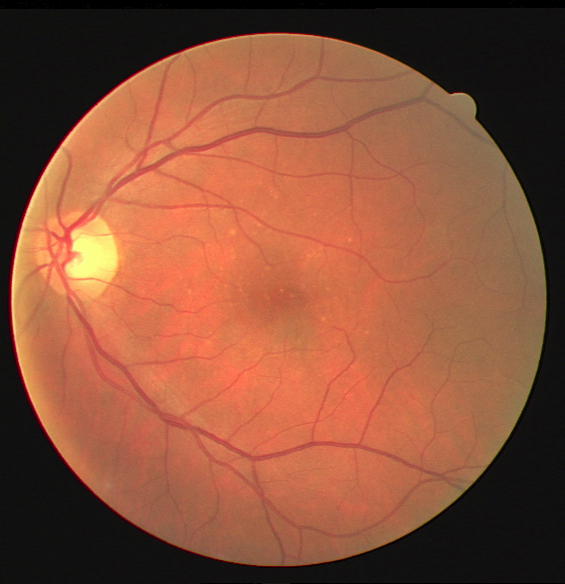
\includegraphics[width=\textwidth]{fundusimage}
		\caption{Fundus Image}
		\label{fig:fundusex}
	\end{subfigure}
	\hfill
	\begin{subfigure}[b]{0.45\textwidth}
		\centering
		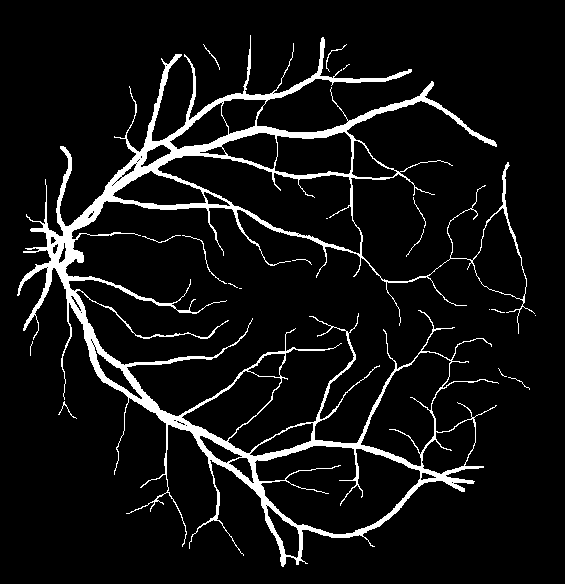
\includegraphics[width=\textwidth]{fundusimageseg}
		\caption{Segmented Vessels}
		\label{fig:fundusex seg}
	\end{subfigure}
	\caption{Fundus Image and its segmentation}
	\label{fig:fundus example}
\end{figure}

The aim of our thesis is to learn a function F which maps the image to its segmentation as, $ F: I \rightarrow S $, i.e, we want to learn a function to segment the vessel in a given fundus image. Inspired by the work of \cite{mnih2012learning, lim2013sketch} we approach the problem of predicting segmentation maps in a  patch based framework. In this patch level method, to predict the segmentation map for an image I, we decompose the image into overlapping patches and predict the segmentation maps for individual patches in a patch by patch fashion. The image and the segmentation map after decomposition can be represented as in Equation \ref{eq:dataset}. Here 'I' denotes the fundus image and 'S' its segmentation map. \\

At the test time, we compute the patches for a given imaget and the mapping function F is then used to predict the segmentation map for all the test patches. Finally, the output segmentation patches are combined by averaging, resulting in an output segmented image. As the patches are computed in an overlapping way, to each pixel several segmentation patches are added during reconstruction phase. More precisely, each pixel is composed of N pixel values from N nearby patches.\\

\subsection{Learning Architecture}
The major part of our work is to learn an effective mapping function F, to map the fundus image to its segmentation map. In both of our models we learn local structure representations in form of a dictionary. This dictionary is composed of patches representing the edge structures, T- junctions, crossovers, parallel lines and other commonly occurring local patterns. To these patches is associated their ground truth segmentations. At prediction time, we then approximately decompose each patch as a linear combination of dictionary elements. To compute the final segmentation of the patch, each atom of the dictionary element in the linear combination is replaced by its segmentation.\\

An example of the learning model is shown in figure \ref{fig:trainmodel}. Both of the models presented in the section, learn this dictionary for predicting the ground truth map.
Before we delve into our models, we list the common preprocessing operations on the input data.
\begin{figure}
	\centering	
	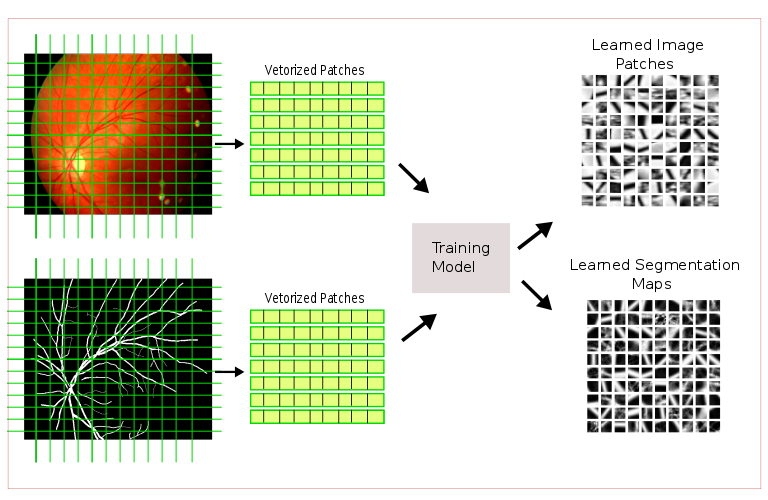
\includegraphics[width=0.8\textwidth]{trainmodel.png}
	\caption{Training architecture for our learning model.}
	\label{fig:trainmodel}		
\end{figure}
\subsubsection{Preprocessing}
For our task we have explored some of the preprocessing steps including patch normalization, contrast stretching and local contrast normalization. For all the experiments, we normalize each input patch by subtracting the patch mean and dividing by the standard deviation per patch. Also, all the input patches are vectorized before being fed to the predictor.


%%%%%%%%%%%%%%%%%%%%%%%%%%%%%%%%%%%%%%%%%%%%%%%%%%%%%%%%%%

\section{Cluster Learning}
In this model we find common local structures within the data using clustering. Image patches are clustered to find a common set of locally appearing structures within the image. As we know the ground truth annotations associated to each image patch, we find the segmentation maps for our clustered structures by associating each segmentation image patch to its corresponding cluster. In this way we learn a dictionary in the form of \{image patch : segmentation\} which is then used to find segmentation map for new patches. This method is inspired in part by work of \citet{lim2013sketch} where they learn commonly occurring structures by clustering on annotated segmentation patches.\\
We call our method as 'Cluster Based - Common Local Structures(CB-CLS)'. Figure \ref{fig:cb-cls} shows an example of learned dictionary on drive dataset.

In the next section we describe in detail the implementation of learning and prediction steps of our algorithm.

\subsection{Learning}

The training procedure for our method requires learning clusters within the input patches. Training is performed on the patches drawn from the input images $I_1$,$I_2$,...$I_n$ and corresponding segmentation images $S_1$,$S_2$,...$S_n$. 

From the training images, we compute a random subset of m patches of fixed size $\sqrt{n}$ x $\sqrt{n}$ and their corresponding annotation as computed from the segmentation images. This subset of patches is used to learn a representative dictionary of patches representing the locally occurring structures in the image and the associated segmentation maps. Let us denote a patch as $x_i$ and its corresponding segmentation map patch as $y_i$. Then the new training set can be represented as:

$$
X = \{x_1,x_2,....,x_n\}
$$
$$
Y = \{y_1,y_2,....,y_n\}
$$
\\
In the next step we find 'k' clusters within the patches in X using K-Means clustering as explained in \ref{sec:kmeans}. Let the 'k' learned cluster be denoted as $C = \{C_1,C_2,...,C_k\} $ where the clusters then can be represented by their cluster centroids $c_1, c_2,..., c_k$. A cluster with 'm' patches then can be represented as

$$
C_k = \{x^k_1,x^k_2,....,x^k_m\}
$$

Now, since we know the annotation $y_i$ for each training patch $x_i$, the image patches in each cluster can be replaced with their corresponding annotation patches to obtain a group of segmentation cluster where each such cluster can be represented as:
$$
SC_k = \{y^k_1,y^k_2,....,y^k_m\}
$$

We then represent each segmentation cluster by the average of all the points within that cluster, found as:
$$	
sc_k = \frac{1}{m}\sum\limits_{i=1}^{m} y^k_m
$$

Finally, we obtain a dictionary which maps the image cluster to a ground truth segmentation patch.
$$
D = \{ (C_k : sc_k) | k =1..m\}
$$

An example of a learned dictionary over image patches on DRIVE dataset is showin in Figure \ref{fig:cb-cls}
\begin{figure}
	\begin{subfigure}[b]{0.45\textwidth}
		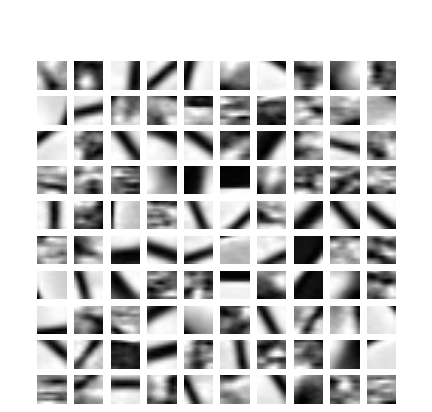
\includegraphics[width=\textwidth]{cluscenters}
		\caption{Learned cluster centers.}
		\label{fig:cluscenters}
	\end{subfigure}
	%
	\begin{subfigure}[b]{0.45\textwidth}
		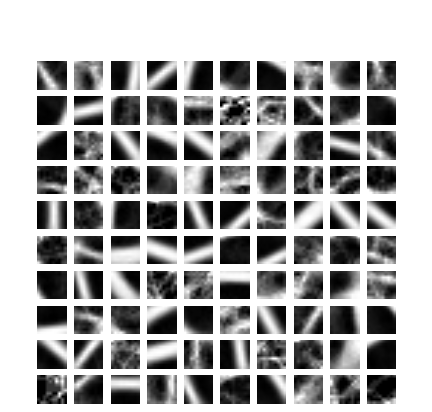
\includegraphics[width=\textwidth]{gtclusters1}
		\caption{Segmentation maps for learned clusters.}
		\label{fig:gtclusters}
	\end{subfigure}
	\caption[Local structures learned using clustering and their segmentation maps]{The image on the left shows the local structures appearing in the images. We can see a mix of straight lines at different orientations and other complex structures. The vessels are in black. The image on the right depicts the corresponding vessels. Vessel pixels are in white and the background in black.}
	\label{fig:cb-cls}
\end{figure}

\subsection{Prediction}
At test time, to predict the segmentation map for an image, we start by extracting dense patches centered at all pixel in the image. For each extracted patch its cluster membership is predicted using the already trained clustering model. The cluster labels are then matched in the dictionary to obtain the respective segmentation map for the patch. Output image is reconstructed from the patch annotations by averaging. 

\subsection{Algorithm}
The entire learning algorithm than can be summarized in following steps:
\begin{enumerate}
	\item Extract a set of random Image-Segmentation patches of size m x m from the training images.
	\item Train a K-Means clustering model on the input image patches and learn k clusters on the input.
	\item Compute the ground truth patch for each cluster by averaging the ground truth annotations for each patch belonging to a cluster. 
	\item Construct a dictionary of Cluster and annotations.
\end{enumerate}


\section{Dictionary Learning}
The model is based on learning an over-complete dictionary over the training data. We aim to learn a good dictionary which can represent our data as a sparse linear combination of the dictionary atoms.
This method is similar to our previous method where also we learn a dictionary which represents the local structures within the data. The mathematical reasoning behind is that, a signal ( in our case an image) can be represented as a combination of a small number of basic structures, like edges and lines.
It is also easy to obtain the segmentation maps for such basic atoms. In our method, for each such image patch, denoted as dictionary atoms, we find a corresponding segmentation label patch from the given segmentation map for the image.\\

For example, given an over complete dictionary of atoms D $\in$ $R^{m,k}$, with k columns as the learned image atoms, we can reconstruct a given image patch x $\in$ $R^m$ as a linear combination of atoms in D. More formally, we learn a sparse code $\alpha$ over D to represent x as

$$ x \approx D \alpha $$  

This is very similar to our cluster based method. The learned cluster centers can be considered as the dictionary with the cluster centers at dictionary atoms. And each point within a cluster can be represented as a linear combination of clusters centers with coefficients $\alpha$, constrained as ${\lVert \alpha \rVert}_0$. This constraint forces our data point to be represented by only one cluster.

The advantage of the dictionary learning method is that it can represent complex structures like t-junctions and crossover regions much more accurately as a combination of various atoms.
As the local structures are learned in dictionaries, we call our method as 'Common Local Structures in Learned Dictionaries(CLS-LD)'
In the following section we describe the implementation of the learning model.

\subsection{Learning}
The learning phase starts by extracting image and label patches from the training data. Let us represent our training set composed of random patches as,
$$
X = \{x_1,x_2,....,x_n\}
$$
$$
Y = \{y_1,y_2,....,y_n\}
$$
where X is composed of image patches and Y the corresponding label patches. Each image patch can be represented as a vector by concatenating each of the pixel values. So given, 'm' patches of size $\sqrt{n}$ x $\sqrt{n}$, the dataset can than be represent as matrices 
X,Y $\in$ $R^{m,n}$. Each row in the matrix denotes a patch or image atom.\\

We learn an over complete dictionary D of basis atoms from the image patches using the dictionary learning methods as described in section \ref{sec:dlsparse}. The aim is to learn a dictionary D with k atoms which can best represent $x_i$ using linear combination of a few atoms $d_k$ of the learned dictionary.

In the next step we learn a sparse code $\alpha$ to represent our input X in terms of dictionary atoms.
$$
X = \alpha D
$$ 
Since we already know the ground truth annotation Y for X, we can infer that Y can be approximately represented as a linear combination of atoms from a dictionary of labels L, corresponding to D.\\

As the sparse code remains same for both the representations, we can compute the dictionary atoms from L by taking a weighted average of all the ground truth patches in Y, weighed by sparse codes for all the patches.\\

So we learn two dictionaries, D of image patches and L consisting of label patches corresponding to atoms in D. An example of the learned dictionaries D and L over DRIVE dataset is shown in figure \ref{fig:dl-cls}

\begin{figure}
	\begin{subfigure}[b]{0.45\textwidth}
		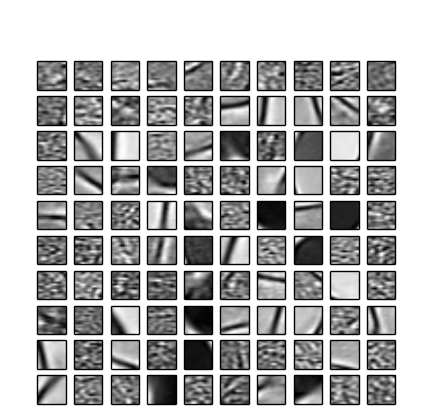
\includegraphics[width=\textwidth]{dict}
		\caption{Dictionary D of atoms learned on the raw image patches}
		\label{fig:dict}
	\end{subfigure}
	%
	\begin{subfigure}[b]{0.45\textwidth}
		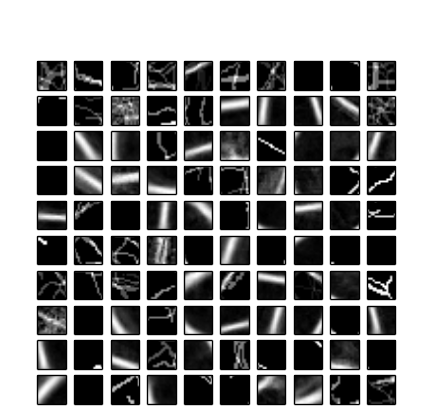
\includegraphics[width=\textwidth]{dict_gt}
		\caption{Dictionary L, consisting of computed segmentation maps for atoms in D}
		\label{fig:dictgt}
	\end{subfigure}
	\caption[Dictionary of image atoms and segmentations]{The image on the left shows the learned representative atoms on raw image patches. Most of the atoms depict simple structures like lines and edges. The vessels are in black. The image on the right depicts the corresponding vessels. Vessel pixels are in white and the background in black.}
	\label{fig:dl-cls}
\end{figure}
\clearpage
\subsection{Prediction}
At the test time, given an image I, dense patches can be computed and the image can be represented as a matrix I $\in$ R, where each row represents a patch of size n x n. We then compute a sparse decomposition of I over dictionary D represented by a sparse code $\alpha$ such that:
$$
I = D \alpha
$$

We can then compute the ground truth segmentation S, for the image patches in I, as :
$$
S = L\alpha
$$
where $\alpha$ is the sparse code computed over dictionary D and L is the label dictionary previously computed during the learning phase.

%%%%%%%%%%%%%%%%%%%%%%%%%%%%%%%%%%%%%%%%%%%%%%%%%%%%%%%%%%
\section{Datasets}
For testing the performance of our algorithm, we train and test our system on the following publicly available datasets. In this section we describe the characteristics of these datasets

\subsection{DRIVE}
The Digital Retinal Images for Vessel Extraction (DRIVE) dataset \cite{drivedataset} consists of 40 color retinal images randomly selected from diabetic retinopathy screening program for 400 diabetic patients. Each of these images in dataset are JPEG compressed and have a dimensions of 768 x 584 pixels captured at a resolution on bits per pixel. The images are captured with a 45degree field of view (FOV).
Of the 40 images in the dataset, 7 show sign of diabetic retinopathy, while the remaining 33 do not consist of any pathology. Each image is provided with a corresponding mask delineating the FOV.\\

The dataset is provided with divisions in terms of training and testing set, with each set consisting of 20 images. Each of the 40 images have been manually segmented by human observers trained by an experienced ophthalmologist. For the training set, single ground truth segmentation of the vessels is provided. The test set is provided with two ground truth segmentations, of which the first one is used as gold standard and the other is used to compare the performance with an independent human observer.\\
\clearpage
\subsection{STARE}
The STARE dataset \cite{hoover2000locating,hoover2003locating} consists of 20 images with blood vessel segmentations, out of which 10 show signs of pathology. The images have been capture with a FOV of 35degrees at 8 bit per pixel resolution, with dimensions of each image as 605 x 700 pixels. The dataset consists of segmentation provided by two human observers. In our experiments, we consider the segmentations provided by the first observer as ground truth.\\

For the experiments, the dataset is randomly divided into training and test sets each consisting of 10 images.

\subsection{ARIA}
The ARIA dataset \cite{farnell2008enhancement, zheng2012automated} consists of three groups of images. One of the group consists of 92 images with age-related macular degeneration, the other with 59 images from diabetic patients and the last group with 61 images from a control group.\\

The images are captures with a 50degree FOV, stored in uncompressed TIFF format, with a resolution of 8bits per pixel. Each image has dimensions of 768 x 576 pixels. The dataset provides with blood vessel segmentation images as manually segmented by experts and a corresponding mask delineating the FOV region.
\clearpage
\subsection{CHASEDB1}
The CHASEDB1 dataset \cite{fraz2012ensemble} consist of 28 images captured at 30degree FOV with a resolution of 1280 x 960 pixels.The dataset consists of two images per patient(one for each eye) captured for 14 children. 

\begin{table}
	\caption{Summary of Datasets}
	\centering
	\label{table:datasets}
	\begin{tabular}{c c c }
		\toprule
		{Datasets} & {FOV} &{\# of Images}  \\ \hline
		
		DRIVE & 45 & 20+20 \\
		
		STARE& 30 & 20  \\
	
		ARIA & 50 & 212 \\
		
		CHASEDB1 & 30 & 28\\
		
		\bottomrule
	\end{tabular}
\end{table}
